\section{Dasar Teori}

Pembuatan proyek akhir ini tentunya merujuk pada beberapa teori dan konsep yang relevan. Studi pustaka ini bertujuan untuk memberikan landasan teoritis yang mendukung pengembangan proyek akhir ini. Beberapa konsep yang menjadi dasar dalam proyek akhir ini antara lain:

\subsection{Hotel Kapsul}

Hotel kapsul adalah jenis akomodasi yang menawarkan ruang tidur kecil dan efisien, biasanya dalam bentuk kapsul atau pod. Konsep ini berasal dari Jepang dan telah menyebar ke berbagai negara di seluruh dunia. Hotel kapsul dirancang untuk memberikan pengalaman menginap yang nyaman dengan harga terjangkau, terutama bagi pelancong yang mencari akomodasi sementara \cite{bobobox}, istilah kamar/room dalam hotel konvensional bila dalam hotel kapsul berubah sesuai dengan bentuknya sebut saja pada platform Tamu.id kamar disebut sebagai Pod, dan dalam satu kapsul hotel terdiri dari beberapa jenis Pod dan tiap jenis pod memiliki spesifikasi dan jumlah Pod yang berbeda-beda.


\subsection{Sistem Informasi}
Sistem informasi adalah kumpulan komponen yang saling berinteraksi untuk mengumpulkan, mengelola, memproses, dan menyebarluaskan informasi guna mendukung pengambilan keputusan yang efektif dan efisien \cite{stair2015}. Sistem informasi terdiri dari beberapa elemen utama, yaitu perangkat keras, perangkat lunak, manusia, data, dan prosedur yang saling berhubungan untuk mencapai tujuan tertentu.

\subsection{Website}
Website adalah sekumpulan halaman web yang saling terhubung dan dapat diakses melalui internet menggunakan protokol HTTP atau HTTPS \cite{mann2016}. Website dirancang untuk menyediakan informasi, layanan, atau hiburan kepada pengguna. Dalam konteks modern, website menjadi elemen penting dalam kehidupan sehari-hari, mulai dari e-commerce, pendidikan, hingga media sosial.

Website terdiri dari dua komponen utama: front-end dan back-end. Front-end mengacu pada tampilan antarmuka pengguna yang dapat diakses melalui browser, sedangkan back-end mencakup server, database, dan logika aplikasi yang mendukung fungsi website tersebut.

Perkembangan teknologi web, seperti HTML5, CSS3, dan JavaScript, telah memungkinkan website menjadi lebih interaktif dan responsif. Selain itu, keberadaan sistem manajemen konten (CMS) seperti WordPress dan Joomla memudahkan pengguna tanpa latar belakang teknis untuk mengelola konten website mereka.

\subsection{OAuth 2.0}
OAuth 2.0 adalah protokol otorisasi yang dirancang untuk memberikan akses terbatas ke sumber daya pengguna di server tanpa perlu membagikan kredensial mereka secara langsung \cite{hardt2012}. Protokol ini biasanya digunakan dalam aplikasi web, perangkat mobile, dan layanan pihak ketiga lainnya.

\begin{figure}[H]
    \centering
    \includesvg[
        width=0.9\textwidth, % Atur lebar sesuai kebutuhan, misal 90% lebar teks
        keepaspectratio % Opsi ini biasanya implisit atau dikelola dengan baik oleh width
    ]{diagram/img/bab2/oauth.svg} % Path ke file SVG Anda, TANPA ekstensi .svg
    \caption{Ilustrasi Protokol OAuth 2.0}
    \label{fig:oauth}
\end{figure}

Seperti pada gambar \ref{fig:oauth}, prinsip kerja OAuth 2.0 melibatkan beberapa entitas, yaitu resource owner (pemilik sumber daya), client (aplikasi pihak ketiga), authorization server (server otorisasi), dan resource server (server sumber daya). Dalam skenario OAuth 2.0, pengguna memberikan izin kepada aplikasi pihak ketiga untuk mengakses data mereka melalui token akses yang diterbitkan oleh server otorisasi.

OAuth 2.0 sering digunakan oleh platform besar seperti Google, Facebook, dan GitHub untuk memungkinkan integrasi dengan layanan mereka. Keamanan dalam OAuth 2.0 sangat bergantung pada implementasi yang benar, termasuk penggunaan HTTPS, pengelolaan token dengan benar, dan mitigasi serangan seperti CSRF.

\subsection{\textit{Webhook}}
Webhook adalah mekanisme komunikasi antara server yang memungkinkan pemberitahuan secara real-time melalui HTTP POST ketika suatu peristiwa tertentu terjadi \cite{jain2021}. Webhook sering digunakan dalam pengintegrasian aplikasi untuk memastikan data tetap sinkron tanpa perlu polling terus-menerus.

Dalam praktiknya, webhook bekerja dengan cara mengirimkan payload berupa data JSON atau XML ke URL tertentu yang telah ditentukan oleh pengguna. Misalnya, layanan pembayaran online dapat menggunakan webhook untuk memberi tahu merchant ketika pembayaran berhasil dilakukan.

Keuntungan utama webhook adalah efisiensi karena server hanya mengirimkan data saat diperlukan, dibandingkan dengan polling yang memeriksa perubahan secara berkala. Namun, implementasi webhook memerlukan pengamanan ekstra untuk mencegah akses tidak sah, seperti menggunakan token validasi atau enkripsi data.

\subsection{\textit{Rest API (Representational State Transfer Application Programming Interface)}}

REST API (Representational State Transfer Application Programming Interface) adalah arsitektur layanan web yang dirancang untuk mendukung komunikasi antara klien dan server melalui protokol HTTP. REST diperkenalkan oleh Roy Fielding dalam disertasinya pada tahun 2000, dengan prinsip utama bahwa setiap sumber daya pada server diidentifikasi melalui URI (Uniform Resource Identifier) \cite{fielding2000}.

\begin{figure}[H]
    \centering
    \includesvg[
        width=0.9\textwidth, % Atur lebar sesuai kebutuhan, misal 90% lebar teks
        keepaspectratio % Opsi ini biasanya implisit atau dikelola dengan baik oleh width
    ]{diagram/img/bab2/rest.svg} % Path ke file SVG Anda, TANPA ekstensi .svg
    \caption{Ilustrasi REST API}
    \label{fig:rest}
\end{figure}

Seperti pada gambar \ref{fig:rest}, REST API memanfaatkan metode HTTP seperti GET, POST, PUT, dan DELETE untuk melakukan operasi pada sumber daya. Pendekatan ini memungkinkan pengembangan layanan web yang skalabel, sederhana, dan mudah diintegrasikan dengan berbagai platform. REST API banyak digunakan dalam pengembangan aplikasi modern karena sifatnya yang ringan dan kompatibel dengan format data seperti JSON dan XML \cite{richardson2007}, Beberapa karakteristik utama REST API meliputi:

\begin{enumerate}
    \item Client-Server: Memisahkan antara klien dan server, memungkinkan evolusi independen dari kedua komponen.
    \item Stateless: Setiap permintaan dari klien ke server harus berisi semua informasi yang dibutuhkan untuk memahami dan memproses permintaan tersebut.
    \item Cacheability: Respons dapat ditandai sebagai dapat di-cache atau tidak untuk mengoptimalkan efisiensi.
    \item Layered System : Klien tidak perlu mengetahui detail implementasi server, memungkinkan fleksibilitas arsitektur.
\end{enumerate}

REST API telah menjadi standar de facto untuk menghubungkan berbagai aplikasi, terutama dalam ekosistem aplikasi berbasis cloud dan microservices \cite{tilkov2010}.

\subsection{\textit{Software Development Life Cycle} dengan Metode \textit{Kanban Board}}

\textit{Software Development Life Cycle} (SDLC) adalah kerangka kerja sistematis untuk merencanakan, membangun, menguji, dan memelihara perangkat lunak. Dalam penelitian ini, alur kerja pengembangan dikelola menggunakan metode \textit{Kanban Board}, yang menekankan pada pengelolaan tugas secara visual, efisien, dan adaptif terhadap perubahan kebutuhan.

\textit{Kanban Board} menyediakan pendekatan visual dalam mengelola tugas melalui tiga kolom utama: \textit{To Do}, \textit{In Progress}, dan \textit{Complete}. Setiap tugas direpresentasikan sebagai kartu yang berpindah antar kolom sesuai dengan statusnya. Pendekatan ini membantu membatasi pekerjaan yang berjalan secara bersamaan (\textit{Work In Progress/WIP}), menjaga aliran kerja yang berkelanjutan, serta memberikan transparansi terhadap progres proyek \cite{anderson2010}.

Penerapan \textit{Kanban Board} dalam SDLC dilakukan secara bertahap, dimulai dari penempatan aktivitas seperti analisis kebutuhan dan perancangan sistem pada kolom \textit{To Do}, pengembangan fitur pada \textit{In Progress}, hingga penyelesaian tugas yang dipindahkan ke kolom \textit{Complete}. Skema ini mendukung proses pengembangan perangkat lunak yang lebih terstruktur, dapat dipantau dengan mudah, dan memungkinkan perbaikan berkelanjutan berdasarkan evaluasi yang dilakukan secara berkala \cite{burrows2014}.


\subsection{Unified Modeling Language (UML)}

Unified Modeling Language (UML) merupakan bahasa pemodelan standar yang digunakan untuk menentukan, memvisualisasikan, membangun, dan mendokumentasikan artefak perangkat lunak serta sistem lainnya. UML memfasilitasi pemahaman antar tim dalam proses pengembangan dengan menyediakan serangkaian notasi yang konsisten dan formal. Komponen utama dalam UML mencakup diagram struktural seperti diagram kelas dan diagram komponen, serta diagram perilaku seperti diagram aktivitas dan diagram use case. UML dirancang untuk mendukung berbagai metodologi pengembangan perangkat lunak dan menjadi alat penting dalam rekayasa perangkat lunak modern \cite{booch2005unified}.

\subsection{\textit{Use Case Diagram}}

\textit{Use case diagram} digunakan untuk memahami interaksi antara sistem dan aktor, yang merupakan entitas eksternal yang berinteraksi dengan sistem tanpa menjadi bagian dari sistem. Diagram ini menggambarkan fungsi-fungsi utama sistem, yang disebut sebagai use case, serta hubungan antara aktor dan use case. Elemen-elemen dalam use case diagram meliputi aktor, use case, dan hubungan yang menghubungkan keduanya, membantu menyederhanakan representasi kebutuhan fungsional sistem \cite{booch2005unified}, berikut pada tabel \ref{tab:ucd-diagram} adalah notasi yang digunakan pada use case diagram.

\begin{longtable}{|>{\centering\arraybackslash}m{0.2\textwidth}|>{\centering\arraybackslash}m{0.2\textwidth}|m{0.5\textwidth}|}
    \caption{Notasi pada \textit{Use Case Diagram}} \label{tab:ucd-diagram}                                                                                                                                \\
    \hline
    \textbf{Notasi}                                                      & \textbf{Nama} & \textbf{Keterangan}                                                                                             \\
    \hline
    \endfirsthead

    \endhead
    \hline
    \endfoot

    \endlastfoot

    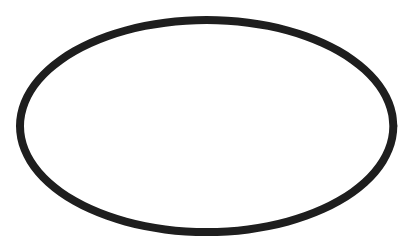
\includegraphics[width=0.2\textwidth]{images/ucd/usecase.png}        &
    \textit{Use Case}                                                    &
    Mewakili serangkaian langkah atau fungsi yang dijalankan sistem untuk menghasilkan nilai atau hasil yang dirasakan oleh aktor. Digunakan untuk menggambarkan perilaku sistem dari perspektif pengguna. \\
    \hline

    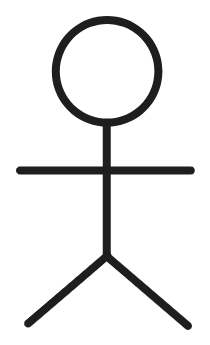
\includegraphics[width=0.1\textwidth]{images/ucd/actor.png}          &
    \textit{Actor}                                                       &
    Entitas eksternal (manusia atau sistem lain) yang berinteraksi dengan sistem. Aktor menjalankan peran tertentu dalam kaitannya dengan satu atau lebih use case.                                        \\
    \hline

    
\includegraphics[width=0.2\textwidth]{images/ucd/association.png}    &
    \textit{Association}                                                 &
    Garis yang menghubungkan aktor dengan use case untuk menunjukkan adanya interaksi atau komunikasi di antara keduanya.                                                                                  \\
    \hline

    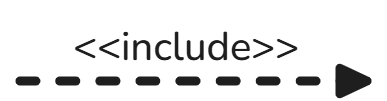
\includegraphics[width=0.2\textwidth]{images/ucd/include.png}        &
    \textit{Include}                                                     &
    Hubungan yang menunjukkan bahwa suatu use case selalu menyertakan perilaku dari use case lain. Digunakan untuk memecah use case kompleks menjadi bagian yang lebih kecil dan dapat digunakan ulang.    \\
    \hline

    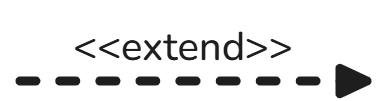
\includegraphics[width=0.2\textwidth]{images/ucd/extend.png}         &
    \textit{Extend}                                                      &
    Menunjukkan bahwa suatu use case dapat memperluas perilaku use case lain secara opsional, tergantung pada kondisi tertentu. Cocok untuk skenario tambahan atau pengecualian.                           \\
    \hline

    
\includegraphics[width=0.2\textwidth]{images/ucd/system.png}         &
    \textit{System Boundary}                                             &
    Kotak atau bingkai yang membatasi cakupan sistem. Semua use case yang ada di dalamnya merupakan bagian dari sistem yang sedang dimodelkan.                                                             \\
    \hline

    
\includegraphics[width=0.2\textwidth]{images/ucd/generalization.png} &
    \textit{Generalization}                                              &
    Menggambarkan hubungan pewarisan antar aktor atau use case. Aktor atau use case anak mewarisi perilaku dari induknya, dan dapat menambahkan perilaku khusus.                                           \\
    \hline

    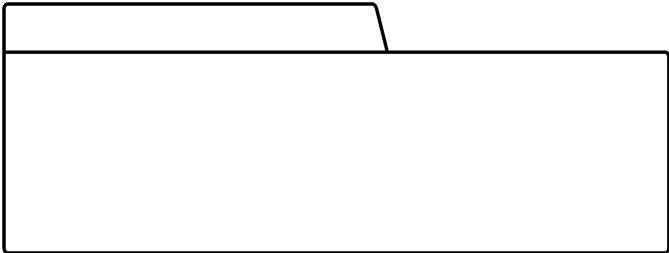
\includegraphics[width=0.2\textwidth]{images/dd/package.png}         &
    \textit{Package}                                                     &
    Digunakan untuk mengelompokkan elemen-elemen dalam diagram agar lebih modular, terstruktur, dan mudah dipahami. Cocok saat sistem kompleks dan terdiri dari banyak komponen.                           \\
    \hline

    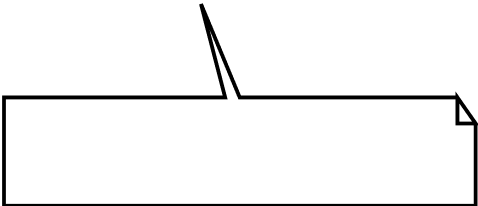
\includegraphics[width=0.2\textwidth]{images/dd/comment.png}         &
    \textit{Comment}                                                     &
    Memberikan penjelasan tambahan atau catatan khusus yang tidak tergambar langsung dari simbol diagram. Membantu dokumentasi dan pemahaman konteks sistem.                                               \\
    \hline
\end{longtable}

\subsection{\textit{Activity Diagram}}

Activity diagram digunakan untuk menggambarkan alur kerja atau proses bisnis dalam suatu sistem. Diagram ini menampilkan aktivitas-aktivitas yang dilakukan dan urutan alurnya. Setiap aktivitas merepresentasikan tindakan tertentu yang dilakukan oleh aktor atau sistem. Elemen penting dalam activity diagram meliputi nodes (kegiatan atau tindakan), edges (aliran), decision points, dan forks. Diagram ini sangat bermanfaat untuk menganalisis alur proses dan mengidentifikasi area untuk optimasi \cite{rumbaugh2005uml}, berikut pada tabel \ref{tab:activity-diagram} adalah notasi yang digunakan pada activity diagram.

\begin{longtable}{|>{\centering\arraybackslash}m{0.2\textwidth}|>{\centering\arraybackslash}m{0.2\textwidth}|m{0.5\textwidth}|}
    \caption{Notasi pada \textit{Activity Diagram}} \label{tab:activity-diagram}                                                                                           \\
    \hline
    \textbf{Notasi}                                                   & \textbf{Nama} & \textbf{Keterangan}                                                                \\
    \hline
    \endfirsthead

    \endhead
    \hline
    \endfoot

    \endlastfoot

    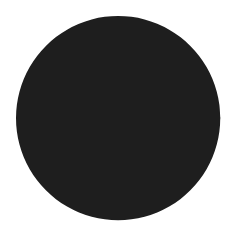
\includegraphics[width=0.1\textwidth]{images/ad/initial-node.png} &
    \textit{Initial Node}                                             &
    Menandai titik awal dari sebuah proses atau aktivitas dalam diagram. Hanya ada satu initial node dalam satu alur proses.                                               \\
    \hline

    
\includegraphics[width=0.1\textwidth]{images/ad/final-node.png}   &
    \textit{Final Node}                                               &
    Menunjukkan titik akhir dari keseluruhan proses. Alur aktivitas berhenti sepenuhnya saat mencapai elemen ini.                                                          \\
    \hline

    
\includegraphics[width=0.2\textwidth]{images/ad/activity.png}     &
    \textit{Activity}                                                 &
    Merepresentasikan satu aksi, langkah, atau tugas spesifik yang dilakukan dalam alur kerja sistem atau pengguna.                                                        \\
    \hline

    
\includegraphics[width=0.2\textwidth]{images/ad/condition.png}    &
    \textit{Decision/Condition}                                       &
    Menggambarkan percabangan alur berdasarkan kondisi tertentu. Setiap cabang berasal dari keputusan logis (true/false atau pilihan lain).                                \\
    \hline

    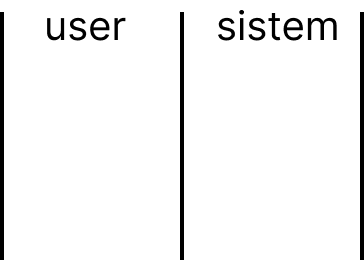
\includegraphics[width=0.2\textwidth]{images/ad/swimlane.png}     &
    \textit{Swimlane}                                                 &
    Membagi aktivitas berdasarkan pelaku atau unit yang bertanggung jawab, seperti pengguna, sistem, atau komponen lainnya. Membantu memperjelas siapa yang melakukan apa. \\
    \hline
\end{longtable}



\subsection{\textit{Entities Relationship Diagram (ERD)}}

Entity Relationship Diagram (ERD) digunakan untuk memodelkan struktur data dalam suatu sistem. Diagram ini merepresentasikan entitas, atribut, dan hubungan antar entitas. Entitas biasanya digambarkan sebagai persegi panjang, atribut sebagai elips, dan hubungan sebagai belah ketupat. ERD membantu memvisualisasikan bagaimana data diatur dan dihubungkan, mempermudah perancangan database secara terstruktur \cite{connolly2005database}, berikut pada tabel \ref{tab:erd-diagram} adalah notasi yang digunakan pada ERD.

\begin{longtable}{|>{\centering\arraybackslash}m{0.2\textwidth}|>{\centering\arraybackslash}m{0.2\textwidth}|m{0.5\textwidth}|}
    \caption{Notasi pada \textit{Entity Relationship Diagram (ERD)}} \label{tab:erd-diagram}                                                                                                   \\
    \hline
    \textbf{Notasi}                                                   & \textbf{Nama} & \textbf{Keterangan}                                                                                    \\
    \hline
    \endfirsthead

    \endhead
    \hline
    \endfoot

    \endlastfoot

    
\includegraphics[width=0.2\textwidth]{images/erd/association.png} &
    \textit{Association}                                              &
    Menunjukkan hubungan antara dua entitas dalam sistem. Biasanya digunakan untuk merepresentasikan koneksi logis atau fungsional, seperti "memiliki", "mengelola", atau "terdiri dari".      \\
    \hline

    
\includegraphics[width=0.2\textwidth]{images/erd/entity.png}      &
    \textit{Entity}                                                   &
    Mewakili objek nyata atau abstrak yang memiliki data dan perlu disimpan dalam sistem, seperti pengguna, produk, atau transaksi. Entitas biasanya digambarkan dalam bentuk persegi panjang. \\
    \hline

    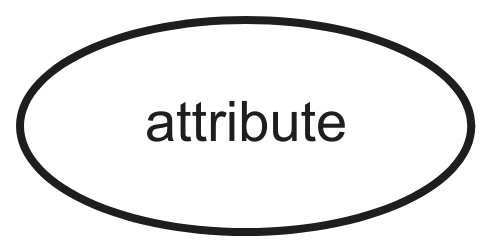
\includegraphics[width=0.2\textwidth]{images/erd/attribute.png}   &
    \textit{Attribute}                                                &
    Menjelaskan detail atau properti dari suatu entitas atau relasi. Contohnya seperti nama, ID, tanggal, yang semuanya menyimpan nilai spesifik untuk setiap instansi entitas.                \\
    \hline

    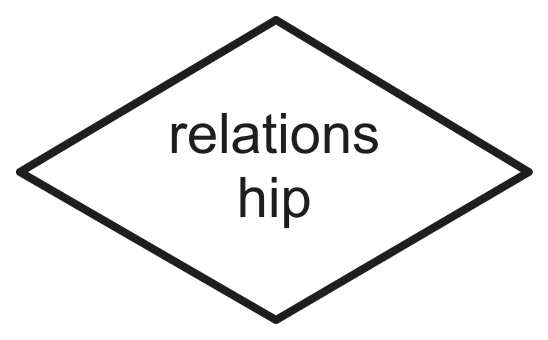
\includegraphics[width=0.2\textwidth]{images/erd/relation.png}    &
    \textit{Relation}                                                 &
    Menyatakan hubungan antar entitas, sering kali dilengkapi dengan kardinalitas (1:1, 1:N, N:N) untuk menunjukkan jumlah keterlibatan antar entitas dalam relasi tersebut.                   \\
    \hline
\end{longtable}


\subsection{\textit{Deployment Diagram}}

Deployment Diagram digunakan untuk menggambarkan bagaimana perangkat lunak di-deploy pada infrastruktur fisik. Diagram ini menunjukkan node (server, perangkat, atau komponen) dan hubungan antar node tersebut. Setiap node dapat memiliki komponen perangkat lunak yang berjalan di atasnya, serta koneksi jaringan yang menghubungkan berbagai node. Deployment Diagram membantu dalam memahami arsitektur sistem dan bagaimana komponen-komponen perangkat lunak berinteraksi dalam lingkungan produksi, berikut pada tabel \ref{tab:deployment-diagram} adalah notasi yang digunakan pada deployment diagram.

\begin{longtable}{|>{\centering\arraybackslash}m{0.2\textwidth}|
    >{\centering\arraybackslash}m{0.2\textwidth}|
    m{0.5\textwidth}|}
    \caption{Notasi pada \textit{Deployment Diagram}} \label{tab:deployment-diagram}                                                                                                                                                                    \\
    \hline
    \textbf{Notasi}                                               & \textbf{Nama} & \textbf{Keterangan}                                                                                                                                                 \\
    \hline
    \endfirsthead
    \endhead
    \endfoot
    \endlastfoot

    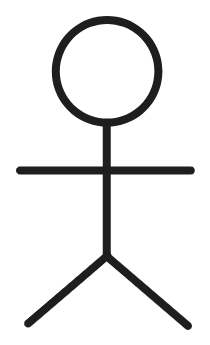
\includegraphics[width=0.1\textwidth]{images/ucd/actor.png}   &
    \textit{Actor}                                                &
    Mewakili entitas eksternal, biasanya manusia, yang berinteraksi dengan sistem. Contohnya pengguna, admin, atau operator.                                                                                                                            \\
    \hline

    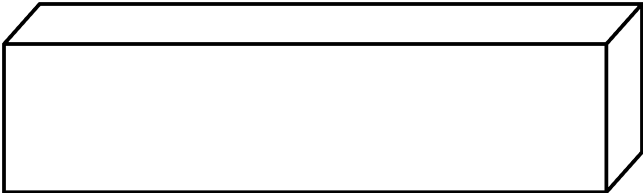
\includegraphics[width=0.2\textwidth]{images/dd/node.png}     &
    \textit{Node}                                                 &
    Menunjukkan perangkat keras, layanan, atau komponen logis tempat proses komputasi berjalan, seperti server, container, atau service.                                                                                                                \\
    \hline

    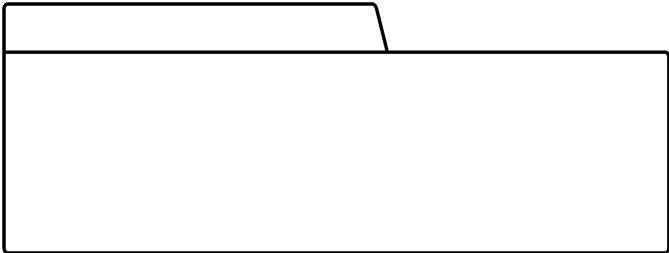
\includegraphics[width=0.2\textwidth]{images/dd/package.png}  &
    \textit{Package}                                              &
    Mengelompokkan beberapa node atau komponen secara logis untuk menyusun arsitektur sistem secara modular dan terstruktur.                                                                                                                            \\
    \hline

    
\includegraphics[width=0.2\textwidth]{images/dd/cloud.png}    &
    \textit{Cloud}                                                &
    Representasi abstrak dari layanan berbasis cloud seperti GCP, AWS, Azure, atau Internet yang menjadi penghubung antar layanan.                                                                                                                      \\
    \hline

    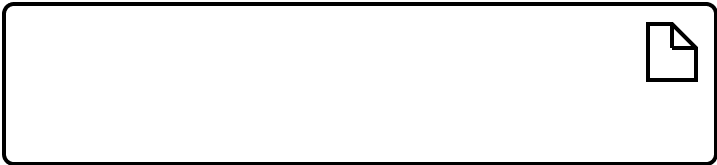
\includegraphics[width=0.2\textwidth]{images/dd/artifact.png} &
    \textit{Artifact}                                             &
    Hasil build atau unit perangkat lunak yang dideploy, seperti aplikasi frontend, backend, skrip konfigurasi, atau file binary.                                                                                                                       \\
    \hline

    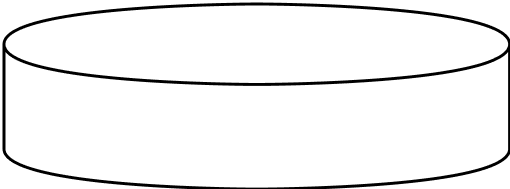
\includegraphics[width=0.2\textwidth]{images/dd/database.png} &
    \textit{Database}                                             &
    Komponen penyimpanan data terstruktur, mewakili sistem manajemen basis data seperti PostgreSQL, MySQL, atau SQLite.                                                                                                                                 \\
    \hline

    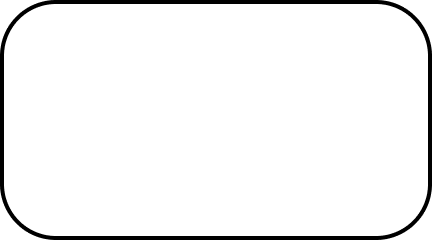
\includegraphics[width=0.2\textwidth]{images/dd/storage.png}  &
    \textit{Storage}                                              &
    Media penyimpanan file atau objek tidak terstruktur, misalnya bucket di Google Cloud Storage, Amazon S3, dan sejenisnya.                                                                                                                            \\
    \hline

    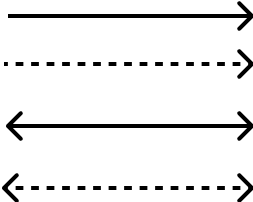
\includegraphics[width=0.2\textwidth]{images/dd/arrow.png}    &
    \textit{Arrow}                                                &
    Digunakan untuk menggambarkan hubungan atau komunikasi antar komponen. Panah solid menunjukkan komunikasi langsung (aktif), panah putus-putus untuk akses pasif (misalnya CDN atau asset fetch), dan panah dua arah mewakili interaksi bolak-balik. \\
    \hline
\end{longtable}


\subsection{\textit{Sequence Diagram}}

Sequence Diagram digunakan untuk menggambarkan interaksi antar objek dalam suatu sistem berdasarkan urutan waktu. Diagram ini menampilkan objek-objek yang terlibat, pesan yang dikirim antar objek, dan urutan eksekusi pesan tersebut. Sequence Diagram membantu dalam memahami bagaimana objek berinteraksi satu sama lain untuk menyelesaikan suatu fungsi atau skenario tertentu, berikut pada tabel \ref{tab:sequence-diagram} adalah notasi yang digunakan pada sequence diagram.

\begin{longtable}{|>{\centering\arraybackslash}m{0.2\textwidth}|
    >{\centering\arraybackslash}m{0.2\textwidth}|
    m{0.5\textwidth}|}
    \caption{Notasi pada \textit{Sequence Diagram}} \label{tab:sequence-diagram}                                                                                                                                                                                       \\
    \hline
    \textbf{Notasi}                                                        & \textbf{Nama} & \textbf{Keterangan}                                                                                                                                                       \\
    \hline
    \endfirsthead
    \endhead
    \endfoot
    \endlastfoot

    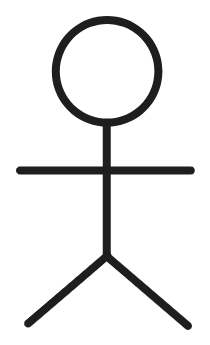
\includegraphics[width=0.1\textwidth]{images/ucd/actor.png}            &
    \textit{Actor}                                                         &
    Mewakili entitas eksternal seperti pengguna atau sistem lain yang memicu interaksi dalam proses yang digambarkan.                                                                                                                                                  \\
    \hline

    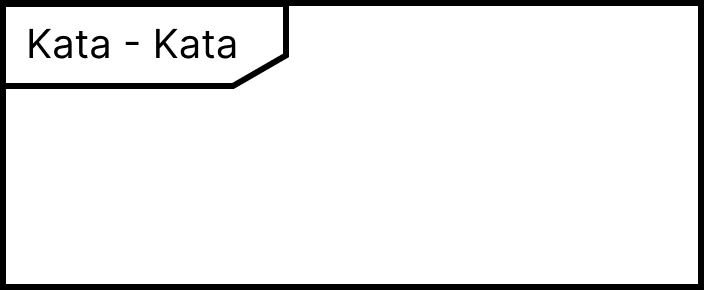
\includegraphics[width=0.2\textwidth]{images/sd/combined-fragment.png} &
    \textit{Combined Fragment}                                             &
    Menyatakan blok kendali alur seperti percabangan, pengulangan, kondisi opsional, dan paralelisme. Label di pojok kiri atas menunjukkan jenis kontrolnya, seperti \textit{opt}, \textit{alt}, \textit{loop}, \textit{par}, dan lainnya.                             \\
    \hline

    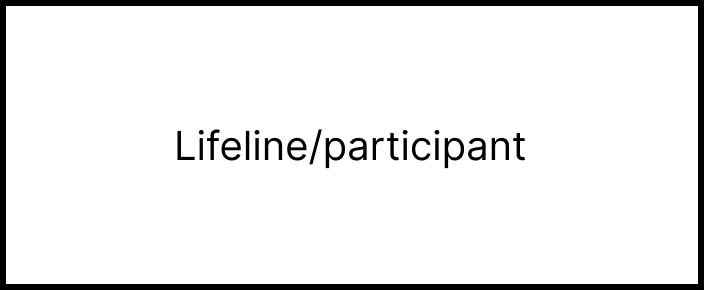
\includegraphics[width=0.2\textwidth]{images/sd/lifeline.png}          &
    \textit{Lifeline/Participant}                                          &
    Representasi objek atau komponen sistem yang terlibat dalam proses, seperti Frontend, Backend, atau API. Digambarkan sebagai garis vertikal yang menunjukkan eksistensinya sepanjang waktu.                                                                        \\
    \hline

    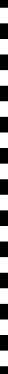
\includegraphics[width=0.006\textwidth]{images/sd/activation.png}      &
    \textit{Activation Bar}                                                &
    Menunjukkan periode di mana sebuah lifeline sedang menjalankan aktivitas atau metode tertentu. Biasanya digambarkan sebagai kotak vertikal tipis.                                                                                                                  \\
    \hline

    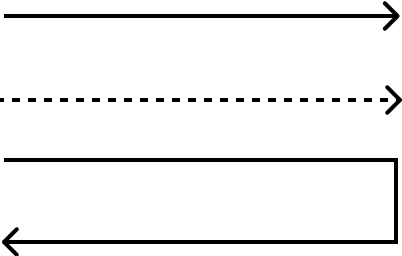
\includegraphics[width=0.2\textwidth]{images/sd/arrow.png}             &
    \textit{Arrow}                                                         &
    Menggambarkan komunikasi atau interaksi antar elemen. Panah solid mewakili permintaan (sinkron), panah putus-putus merepresentasikan respons atau hasil (asinkron), dan panah melengkung digunakan untuk pemanggilan metode pada objek itu sendiri (self-message). \\
    \hline

    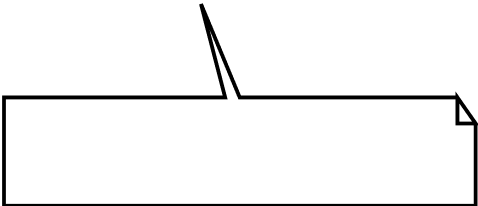
\includegraphics[width=0.2\textwidth]{images/dd/comment.png}           &
    \textit{Comment}                                                       &
    Menyediakan keterangan tambahan yang tidak direpresentasikan secara eksplisit dalam notasi diagram, guna memperjelas konteks atau penjelasan proses tertentu.                                                                                                      \\
    \hline
\end{longtable}





\subsection{Teknologi dan Kakas Pengembangan}

Dalam pengembangan proyek akhir ini, penulis menggunakan beberapa teknologi dan kakas pengembangan yang mendukung proses pengembangan. Beberapa teknologi dan kakas pengembangan yang digunakan antara lain:

\begin{itemize}
    \item \textbf{VueJS}: VueJS adalah pustaka JavaScript yang digunakan untuk membangun antarmuka pengguna yang interaktif dan responsif. VueJS menggunakan konsep komponen yang dapat digunakan kembali untuk memisahkan tampilan dari logika aplikasi, memungkinkan pengembangan yang lebih efisien dan mudah diatur \cite{vuedocs}.

    \item \textbf{Python}: Python adalah bahasa pemrograman tingkat tinggi yang digunakan untuk pengembangan aplikasi web, analisis data, dan kecerdasan buatan. Python memiliki sintaks yang sederhana dan mudah dipahami, serta mendukung berbagai pustaka dan kerangka kerja yang mempermudah pengembangan perangkat lunak \cite{python}.

    \item \textbf{Flask}: Flask adalah kerangka kerja web berbasis Python yang digunakan untuk membangun aplikasi web dan API. Flask dirancang untuk menjadi ringan dan fleksibel, memungkinkan pengembang untuk memilih komponen yang sesuai dengan kebutuhan proyek mereka. Flask juga mendukung berbagai ekstensi yang mempermudah pengembangan aplikasi web \cite{flask}.

    \item \textbf{PostgreSQL}: PostgreSQL adalah sistem manajemen basis data relasional (RDBMS) open-source yang digunakan untuk menyimpan dan mengelola data. PostgreSQL mendukung berbagai fitur seperti transaksi, indeks, dan fungsi yang memungkinkan pengembang untuk membangun aplikasi yang aman dan efisien \cite{postgresql}.

    \item \textbf{Git}: Git adalah sistem kontrol versi yang digunakan untuk mengelola perubahan kode sumber dalam pengembangan perangkat lunak. Git memungkinkan pengembang untuk bekerja secara kolaboratif, melacak perubahan kode, dan mengelola versi kode dengan mudah \cite{git}.

    \item \textbf{GitLab}: GitLab adalah platform pengembangan perangkat lunak berbasis Git yang menyediakan repositori kode, manajemen proyek, dan alat kolaborasi untuk tim pengembang. GitLab memungkinkan pengembang untuk menyimpan kode sumber, melacak masalah, dan berkolaborasi dalam proyek secara efisien \cite{gitlab}.

    \item \textbf{Visual Studio Code}: Visual Studio Code adalah editor kode sumber ringan dan kuat yang dikembangkan oleh Microsoft. Visual Studio Code menyediakan berbagai fitur seperti penyorotan sintaks, debugging, dan ekstensi yang mempermudah pengembangan perangkat lunak \cite{vscode}.

    \item \textbf{Google Cloud Run}: Google Cloud Run adalah layanan komputasi tanpa server yang memungkinkan pengembang untuk menjalankan aplikasi kontainer di infrastruktur Google Cloud. Cloud Run secara otomatis mengelola skala dan sumber daya yang dibutuhkan untuk menjalankan aplikasi, memungkinkan pengembang untuk fokus pada pengembangan tanpa perlu khawatir tentang manajemen infrastruktur \cite{cloudrun}.

    \item \textbf{Hoppscotch}: hoppscotch adalah aplikasi web open-source yang digunakan untuk menguji dan mengelola API. hoppscotch menyediakan antarmuka yang intuitif dan mudah digunakan untuk membuat dan mengirim permintaan HTTP ke API, serta melihat respons yang dihasilkan \cite{hoppscotch}.

    \item \textbf{JSON Web Token (JWT)}: JSON Web Token (JWT) adalah standar terbuka yang digunakan untuk membuat token akses yang aman dan dapat diverifikasi. JWT digunakan dalam aplikasi web modern untuk otentikasi dan otorisasi pengguna, serta pertukaran informasi yang aman antara klien dan server \cite{jwt}.

    \item \textbf{SQLAlchemy}: SQLAlchemy adalah ORM (Object-Relational Mapping) yang digunakan untuk menghubungkan aplikasi Backend python yang mengunakan Flask dengan basis data. SQLAlchemy menyediakan API yang intuitif dan deklaratif untuk berinteraksi dengan basis data, memungkinkan pengembang untuk fokus pada logika aplikasi tanpa perlu menulis query SQL secara manual \cite{sqlaclhemy}.

    \item \textbf{Google Cloud Storage}: Google Cloud Storage adalah server penyimpanan objek (object storage) yang merupakan salah satu lini produk dari google cloud \cite{gcs}.

    \item \textbf{Docker}: Docker adalah platform open-source yang digunakan untuk mengemas, mengirim, dan menjalankan aplikasi dalam kontainer. Docker memungkinkan pengembang untuk membuat lingkungan yang konsisten dan portabel untuk aplikasi, serta mempercepat siklus pengembangan dan penyebaran aplikasi \cite{docker}.

          % \item \textbf{K6}: K6 adalah alat pengujian beban open-source yang digunakan untuk menguji kinerja aplikasi web dan API. K6 menyediakan skrip pengujian yang mudah digunakan dan hasil pengujian yang terperinci, memungkinkan pengembang untuk mengidentifikasi dan memperbaiki masalah kinerja dengan cepat \cite{k6}.

    \item \textbf{Latex}: Latex adalah sistem penyiapan dokumen yang digunakan untuk membuat dokumen yang berkualitas tinggi, seperti artikel ilmiah, laporan, dan buku. Latex menggunakan sintaks markup untuk mengatur struktur dokumen, memungkinkan pengembang untuk fokus pada konten tanpa perlu khawatir tentang tata letak \cite{latex}.
\end{itemize}

\subsection{Pengujian Sistem}

Setelah pengembangan sistem selesai, langkah selanjutnya adalah melakukan pengujian untuk memastikan bahwa sistem berfungsi dengan baik dan sesuai dengan kebutuhan pengguna. Pengujian sistem adalah proses verifikasi dan validasi yang dilakukan untuk mengevaluasi kualitas sistem dan memastikan bahwa sistem memenuhi spesifikasi yang telah ditentukan. Beberapa jenis pengujian sistem yang umum dilakukan antara lain:

\begin{enumerate}
    \item  \textbf{Pengujian Black Box}: Pengujian ini berfokus pada validasi fungsionalitas sistem tanpa memperhatikan struktur internal atau kode sumbernya. Tujuan utama dari pengujian ini adalah untuk memastikan bahwa masukan (input) menghasilkan keluaran (output) yang sesuai dengan spesifikasi \cite{pressman2014}.

          % \item \textbf{Pengujian Beban} : Pengujian beban dilakukan untuk mengevaluasi kinerja sistem di bawah kondisi beban tertentu, seperti jumlah pengguna atau permintaan data yang tinggi. Tujuannya adalah untuk memastikan sistem dapat menangani beban kerja yang diharapkan tanpa mengalami penurunan performa secara signifikan \cite{patton2006}.

    \item \textbf{User Acceptance Testing (UAT)} : UAT adalah tahap akhir pengujian yang melibatkan pengguna akhir untuk memastikan bahwa sistem memenuhi kebutuhan bisnis dan dapat digunakan sebagaimana mestinya. Pada UAT, setiap fungsi sistem diuji berdasarkan skenario yang dirancang sesuai dengan kebutuhan pengguna \cite{mathur2017}. Tingkat keberhasilan UAT dapat dihitung dengan rumus berikut:

          \begin{table}[H]
              \centering
              \begin{tabular}{|c|c|}
                  \hline
                  \textbf{Jawaban}         & \textbf{Bobot} \\ \hline
                  Sangat Setuju(SS)        & 5              \\ \hline
                  Setuju(S)                & 4              \\ \hline
                  Cukup Setuju(CS)         & 3              \\ \hline
                  Tidak Setuju(TS)         & 2              \\ \hline
                  Sangat Tidak Setuju(STS) & 1              \\ \hline
              \end{tabular}
              \caption{Bobot Jawaban \textit{UAT} berdasarkan skala \textit{Likert}}
              \label{tabel:bobot-jawaban-uat}
          \end{table}

          Penentuan skor UAT dihitung menggunakan rumus pada Persamaan \ref{eq:uat} dan hasil dari Skor tersebut akan dibandingkan dengan pengelompokkan pada tabel \ref{tabel:bobot-jawaban-uat} berdasarkan skala \textit{Likert}.


          \begin{equation}
              \label{eq:uat}
              \mathit{Hasil}(\%) = \left(\frac{A}{B \times N}\right) \times 100\%
          \end{equation}

          Keterangan: \\
          A = total skor yang diperoleh dari semua responden \\
          B = maksimum skor yang dapat diperoleh dari setiap responden \\
          N = total responden

          Persentase akhir UAT kemudian dapat dijadikan sebagai indikator kelayakan sesuai kategori yang ditunjukkan pada Tabel \ref{tabel:kategori-kelayakan}.

          \begin{table}[H]
              \centering
              \begin{tabular}{|c|c|c|}
                  \hline
                  \textbf{No.} & \textbf{Skor} & \textbf{Kategori Kelayakan} \\ \hline
                  1.           & $<$ 21\%      & Sangat Tidak Layak          \\ \hline
                  2.           & 21-40\%       & Tidak Layak                 \\ \hline
                  3.           & 41-60\%       & Cukup Layak                 \\ \hline
                  4.           & 61-80\%       & Layak                       \\ \hline
                  5.           & 81-100\%      & Sangat Layak                \\ \hline
              \end{tabular}
              \caption{Kategori Kelayakan UAT}
              \label{tabel:kategori-kelayakan}
          \end{table}

\end{enumerate}